\chapter{Rectification}
\label{ch:rectenna}

\section{Goals of Rectenna}
\label{sec:rectenna-goals}

One of the main components of any WPT system is its rectifier, as it performs the crucial step of capturing the broadcasted energy and transforming it into a usable form. To accomplish this, a rectenna, a dual-purpose device that combines an antenna and a rectifier, is necessary. The antenna picks up the unusable, oscillating AC signal received from the transmitter, the rectifier converts the signal to relatively stable DC power, and this usable power is passed to an arbitrary load.

In addition to standard rectification, the rectenna must serve as a passive nonlinear element. In NLTR, a nonlinear element is required to produce harmonics from the initial interrogation pulse broadcast by the transmitter. However, this goal is secondary to the main purpose of rectification.

The rectenna was designed to fit the following parameters. First, the rectenna must operate efficiently at the high frequency (\numrange{1}{10}~GHz) required for efficient NLTR. Additionally, losses due to reflection and parasitic effects within the antenna should be minimized. Finally, to fulfill the role of a nonlinear element, the rectenna should generate distinguishable harmonics strong enough for the purposes of NLTR.

In short, to rectify and generate harmonics for NLTR, the rectenna must be capable of not only efficient rectification at high frequencies, but also production of strong harmonics for NLTR.

\section{Diode Selection and Testing}
\label{sec:rectenna-diode}

The diode is the most important single component to consider for the rectenna, as it is the main rectifying component. Careful consideration of its characteristics is vital. The switching frequency, forward voltage drop, and impedance of the diode are of particular importance to the desired goal of efficient rectification.

For the rectenna in our design to perform efficiently, the diode must satisfy several requirements:

The diode must maintain functionality as a diode at a transmission frequency of \numrange{1}{10}~GHz, and must rectify at a frequency of at least 10 GHz. This requirement severely limits the possible choices for the rectenna diode. The frequency of a diode is inversely related to its reverse-recovery time (TRR), the fastest time the diode can switch from forward to reverse bias~\cite{an1012-TRR}.In traditional P-N junction diodes, minimum TRR is on the order of tens to thousands of nanoseconds, even for fast diodes~\cite{davis2011schottky}. In a high frequency circuit, a P-N diode would be no different than a short circuit, and no rectification would occur.

The diode must have the lowest forward voltage drop possible. The voltage drop represents the reverse bias that remains when the diode works in the forward direction, and can be a significant contributor to power loss. The team's experimental WPT capabilities are limited to fairly low voltage microwave signals (.5 V to 1 V signal amplitude), which makes forward voltage drop especially important.

Finally, impedances should be minimized to reduce loss. All diodes have intrinsic impedances such as parasitic capacitance and resistance. Impedances contribute to losses during rectification and destabilize circuit behavior, resulting in unpredictable behavior.

Considering these factors, a Schottky barrier diode were chosen for the rectenna. Unlike P-N junction diodes, Schottky diodes have extremely low TRR and low forward voltage~\cite{davis2011schottky}.  Schottky diodes do have a lower maximum reverse voltage rating, higher reverse leakage current, and higher cost than P-N diodes. However, these are relatively minor issues in our application. A Schottky \texttt{MA4E1317} diode was used as the rectifying diode. The diode parameters from the are shown in Table~\ref{tab:rectenna-datasheet}.

\def\arraystretch{2}
\begin{table}[h!]
\centering
\begin{tabular}{|c|c|c|c|c|c|}
\hline
\textbf{Test Conditions} & \textbf{Symbol} & \textbf{Units} & \textbf{Min.} & \textbf{Typ.} & \textbf{Max.} \\ \hline
Junction Capacitance at 0 V at 1 MHz & Cj & pF & - & .020 & - \\ \hline
Total Capacitance at 0 V at 1 MHz & Ct & pF & .030 & .045 & .060 \\ \hline
Junction Capacitance Difference & DCj & pF & - & - & - \\ \hline
Series Resistance at +10 $mA^2$ & Rs & $\Omega$ & - & 4 & 7 \\ \hline
Forward Voltage at +1 $mA$ & $Vf_1$ & V & .60 & .70 & .80 \\ \hline
Forward Voltage Difference at +1 $mA$ & DVf & V & - & - & - \\ \hline
Reverse Breakdown Voltage at $-10 \mu A$ & Vbr & V & 4.5 & 7 & - \\ \hline
SSB Noise Figure & NF & dB & - & $6.5^4$ & - \\ \hline
\end{tabular}
\caption[Datasheet for diode used in rectenna construction]{Datasheet for the M/A-Com \texttt{MA4E1317} Schottky diode~\cite{ma4e1317-datasheet}.}
\label{tab:rectenna-datasheet}
\end{table}

The \texttt{MA4E1317} has low total capacitance (.045~pF) and series resistance (4~$\Omega$), minimizing parasitic losses. The datasheet also cites an operating frequency of up to 80 GHz for this diode, more than sufficient for our purposes. The forward voltage cited to be around .7~V, a typical value for most diodes~\cite{ma4e1317-datasheet}. A lower forward voltage would be desirable, and in considering future improvements to the system, this is definitely a point to consider.

\section{Antenna Design}
\label{sec:rectenna-antenna}

A printed circuit board (PCB) half-wave dipole was chosen as the antenna for the system. The copper trace acts as the antenna, and is etched into a FR-4 substrate. The \texttt{MA4E1317} is a flip-chip device, and is only suitable for mounting on a PCB. The design and specific parameters of the antenna is based off of the dual frequency WPT rectenna in~\cite{suh2002high}, but has been modified in our implementation. The design of the rectenna is shown in Figure~\ref{fig:rectenna-design}.


\begin{figure}[h!]
    \centering
    \begin{subfigure}{.85\textwidth}
        \centering
        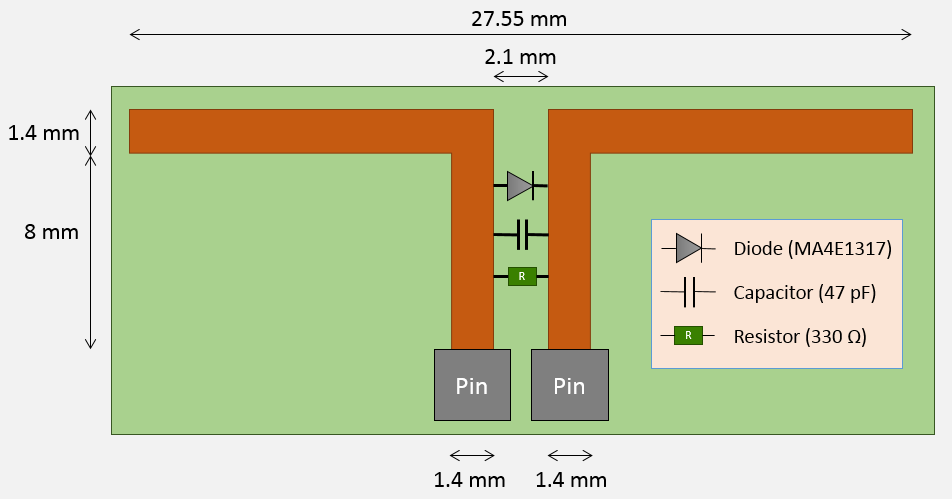
\includegraphics[width=1.0\linewidth]{rectenna/rectenna-design}
        \caption[Rectenna schematica]{A schematic of the PCB rectenna design and component specifications.}
    \end{subfigure}
    \begin{subfigure}{.85\textwidth}
        \centering
        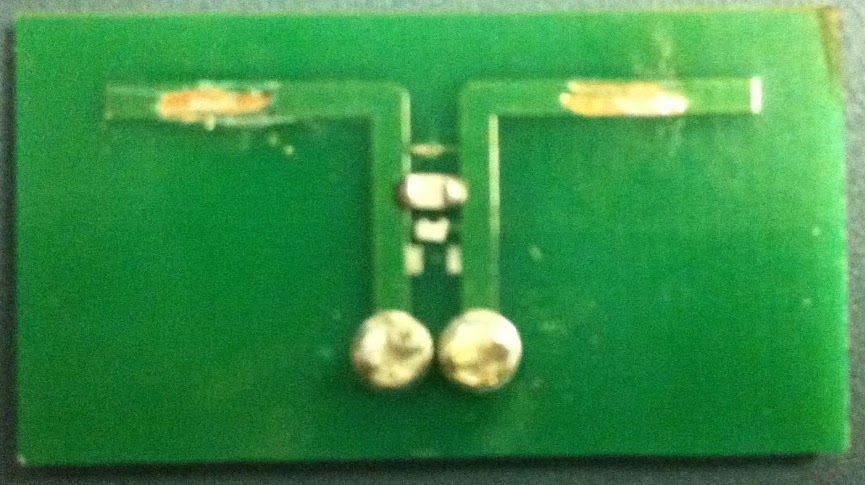
\includegraphics[width=1.0\linewidth]{rectenna/rectenna-photo}
        \caption[Assembled rectenna photo]{Image of the assembled rectenna}
    \end{subfigure}
    \caption[Rectenna design]{Rectenna design}
    \label{fig:rectenna-design}
\end{figure}

The rectenna is composed of the \texttt{MA4E1317} diode, a 47~pF ceramic capacitor acting as a low-pass microwave filter, a 330~$\Omega$ load resistor, and output pins for measurement purposes. The antenna is designed for operation at 5.45~GHz, so the length of the dipole is 27.55~mm, half the wavelength of the incident wave.

One important distinction for this rectenna design is the lack of filtering for higher-order harmonics. This feature is common in most rectennas, but is deliberately left out so that the antenna can generate nonlinear harmonics from the interrogation signal.

No special consideration for impedance matching between the antenna and the rectifier components. This is definitely a point to consider for future improvement, as proper matching of the components should significantly improve the efficiency of rectification.

\section{Rectenna Testing}
\label{sec:rectenna-testing}

To thoroughly test the rectenna, distinct tests were run to order to verify both its rectification and harmonic generation capabilities. We examined a range of frequencies for all tests to isolate peak performance.

\subsection{DC Power Characterization}

To determine the overall rectification efficiency, a second antenna was used to broadcast energy to the rectenna. A 17~dBm~CW signal was generated from the PSG and broadcast through a monopole antenna. The rectenna was then positioned parallel to the broadcast antenna, at a distance of 2~cm. and the average DC voltage and power was measured over the load resistor. The test was repeated over a range of broadcast frequencies from 1~to~7~GHz. The setup is shown in Figure~\ref{fig:rectenna-test-1-setup} and the results are shown in Figure~\ref{fig:rectenna-test-1-voltage}.


\begin{figure}[h!]
    \centering
    \begin{subfigure}{.85\textwidth}
        \centering
        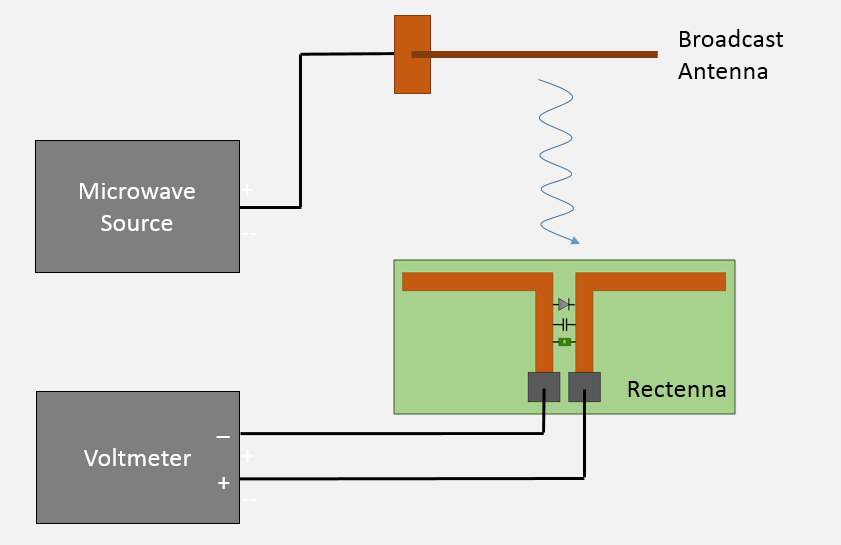
\includegraphics[width=1.0\linewidth]{rectenna/test-1-setup}
        \caption{Experimental setup for rectification testing}
        \label{fig:rectenna-test-1-setup}
    \end{subfigure}
    \begin{subfigure}{.85\textwidth}
        \centering
        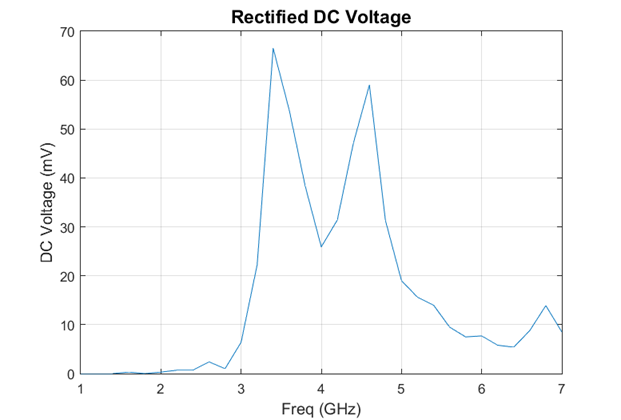
\includegraphics[width=1.0\linewidth]{rectenna/test-1-voltage}
        \caption{DC voltage measured from the voltmeter in the setup on the left for a range (1-7~GHz) of frequency inputs.}
        \label{fig:rectenna-test-1-voltage}
    \end{subfigure}
    \label{fig:rectenna-test-1}
\end{figure}

Rectification was most pronounced in the 3-5~GHz frequency band. Rectified voltage is highest at 3.4~GHz and 4.6~GHz, with DC voltage levels of 66.5~mV and 59.0~mV respectively. Unfortunately, DC voltage results of higher frequencies were unreliable and erratic given the measurement techniques, and accurate data could not be taken.

Given the resistive load of 330~$\Omega$, rectified DC power can be calculated from the voltage above. Using DC voltage ($V$) and load resistance ($R$), the DC power ($P_{dc}$) was calculated using Equation ~\ref{eq:dc_power}:

\begin{equation}
P_{dc} = \frac{V^2}{R}
\label{eq:dc_power}
\end{equation}

A plot of this is shown in Figure~\ref{fig:rectenna-test-1-power}.

\begin{figure}[h!]
\centering
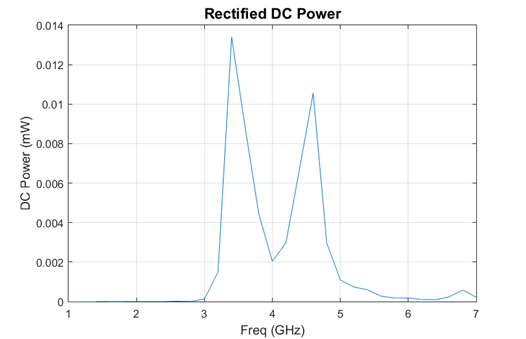
\includegraphics[width=0.85\textwidth]{rectenna/test-1-power}
    \caption[Rectified DC power]{Rectified DC power calculated from DC voltage using the relation: $P = \frac{V^2}{R}$}
    \label{fig:rectenna-test-1-power}
\end{figure}


Considering the input power of 17~dBm (around 50.12~mW), the wall-to-load efficiency of the experiment is extremely low for all frequencies. These losses can come from a number of sources, including bad coupling between the broadcast antenna and rectenna, reflection from broadcast antenna, losses in coaxial connections between components, and power radiated away from the rectenna, among others. However, the inherent losses of the experimental setup are not relevant to the overall efficiency of the system; for this, the efficiency result must be compared to only the rectification efficiency.

To establish rectification efficiency, AC power tests were conducted on a bare dipole antenna with no diode, resistor, or capacitor. The results of this test establish the overall power accepted by the rectenna, and is directly comparable to the previous DC power results.

The setup of the AC power experiment was similar to the DC power experiment, with the exception of two key differences: the voltmeter was replaced by a \texttt{DSO91304A} oscilloscope, and the rectenna was replaced by the bare dipole antenna. In the absence of the 330~$\Omega$ load resistor on the rectenna, the 50~$\Omega$ input impedance of the oscilloscope~\cite{DSO91304A-manual} was used as the load.

Using AC voltage amplitude ($V_{max}$) and load resistance ($R$), the accepted AC power ($P_{ac}$) was calculated using Equation ~\ref{eq:ac_power}:

\begin{equation}
P_{ac} = \frac{V_{max}^2}{2R}
\label{eq:ac_power}
\end{equation}

The setup and results of the test are shown below in Figures~\ref{fig:rectenna-test-2-setup}~and~\ref{fig:rectenna-test-2-power}, respectively.

\begin{figure}[h!]
    \centering
    \begin{subfigure}{.85\textwidth}
        \centering
        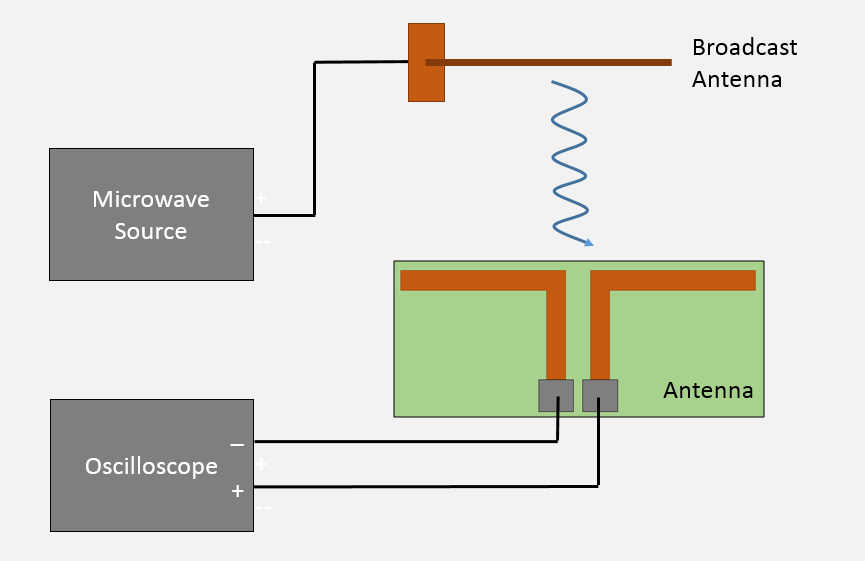
\includegraphics[width=1.0\linewidth]{rectenna/test-2-setup}
        \caption{Experimental setup for measuring accepted AC power}
        \label{fig:rectenna-test-2-setup}
    \end{subfigure}
    \begin{subfigure}{.85\textwidth}
        \centering
        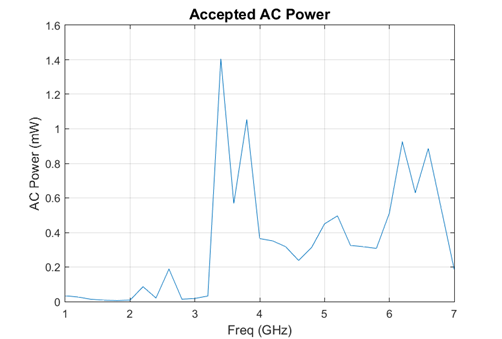
\includegraphics[width=1.0\linewidth]{rectenna/test-2-power}
        \caption[Accepted AC power]{Accepted AC power, used to establish a baseline for efficiency calculation, calculated using the relation $P = \frac{V_{max}^2}{2R}$.}
        \label{fig:rectenna-test-2-power}
    \end{subfigure}
    \label{fig:rectenna-test-2}
\end{figure}

Assuming that the transfer function between the antennas doesn't change between the AC and DC tests, these results allow the rectification efficiency to be calculated. The efficiency ($E$) in this case is the ratio of the rectified DC power ($P_{dc}$) to the total accepted AC power ($P_{dc}$), as in Equation ~\ref{eq:rec_eff}:

\begin{equation}
E = \frac{P_{dc}}{P_{ac}}
\label{eq:rec_eff}
\end{equation}

Figure~\ref{fig:rectenna-efficiency} shows the efficiency calculated this way, across the range of frequencies tested.

\begin{figure}[h!]
\centering
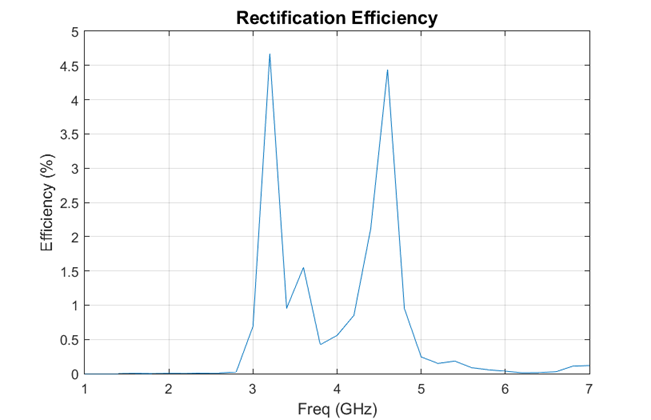
\includegraphics[width=0.85\textwidth]{rectenna/efficiency}
    \caption[Rectification efficiency]{Rectification efficiency, calculated using accepted AC power as a baseline. Calculated using the ratio of rectified DC power to accepted AC power.}
    \label{fig:rectenna-efficiency}
\end{figure}

Analysis of the graph shows the same peak rectification efficiencies at 3.2~GHz and 4.6~GHz, with 4.7\% and 4.4\% respectively. This rather low efficiency is expected given the lack of optimization and impedance matching in the rectenna. However, this result clearly demonstrates rectification of high frequency AC power.

\subsection{Harmonic Generation}

Harmonic generation was then tested by measuring second harmonic power reflected from the rectenna. The antenna was stimulated by a 0~dBm~CW signal, and the second harmonic reflected from the antenna was collected using a directional coupler feeding into the spectrum analyzer for measurement. The test setup for and results are shown in Figure~\ref{fig:rectenna-test-3-setup}.

\begin{figure}[h!]
\centering
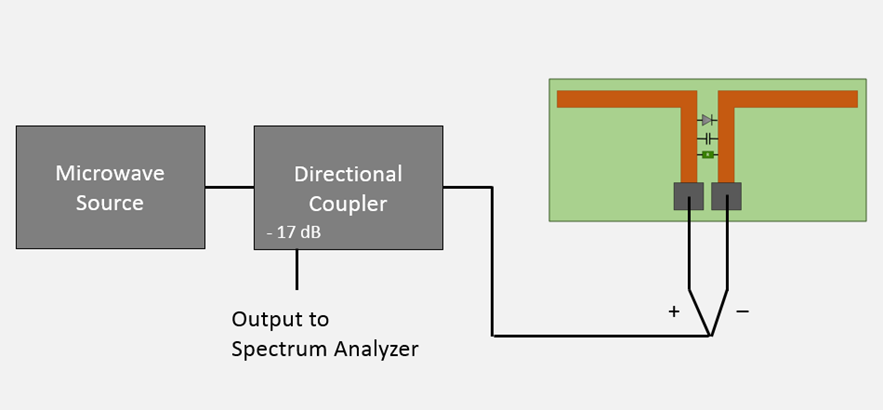
\includegraphics[width=0.85\textwidth]{rectenna/test-3-setup}
\caption{Experimental setup for harmonic generation testing.}
\label{fig:rectenna-test-3-setup}
\end{figure}

In initial testing, the harmonic generation of the rectenna was minimal, as the measured 2nd harmonic power was comparable to the noise level power. However, after filtering out harmonic responses from microwave source, a distinct 2nd harmonic was found at 2.45~GHz at -150~dBm compared to the noise level power of -161~dBm. Bandwidth restrictions of filtering components prevented analysis of a full frequency spectrum, and thus, 2.45~GHz is the only frequency we were able to probe for harmonics. Even so, this result does demonstrate the harmonic generation capabilities of the rectenna.

\section{Discussion}
\label{sec:rectenna-discussion}

The intent of the rectenna was twofold. The rectenna was designed to rectify RF signals (\numrange{1}{10}~GHz) and generate of higher-order harmonics. Both of these qualities are needed for the creation of an NLTR rectifier. The current experiments establish a baseline for rectification and harmonic generation that can be used for future designs.

The current design has made no steps towards the impedance matching of the antenna to the components. This is likely a major source of power lost by the system for rectification, and should be a top priority to consider in subsequent designs.

Our design of a dual-purpose rectenna satisfied our initial goals, and is a first step towards a functioning NLTR based WPT system. After considerable optimization and miniaturization, the rectenna would be used as a receiver for the electronics we want to power. After receiving the initial interrogation pulse and generating the 2nd harmonic response, it would then receive the main high power pulse and rectify the signal, providing the load device with DC power. Due to the nature of NLTR, the receiving devices don’t require power to facilitate the process.
